\part{Clock and Control interface for the Large Pixel Detector} % (fold)
\label{prt:lpd_ccc_interface}

\chapter{Introduction} % (fold)
\label{cha:lpd_ccc_introduction}

\section{Conventions} % (fold)
\label{sec:conventions}
Throughout this document there are several typographical conventions that are observed (see table~\ref{tab:typography}).
% CAPS           = states          e.g. IDLE, 
% bold(CAPS)     = generic         e.g. BUNCH_LENGTH 
% textttt{CAPS}  = commands        e.g. SET_TRIGGER_FLAG
% textttt{lower} = ports/signals   e.g. start_i
% 
% 
% veto from ccc->veto to asic 7 clk
% start from ccc->start to asic 6 clk
% above due to requirements to sync to 4.5 MHz
\begin{table}[htbp]
  \begin{center}
  \begin{tabular}{c|c}
    Type or prefix                  & Meaning                             \\
    \hline                                                   
    \texttt{lower mono-spaced font} & Port or signal names.               \\
    lower normal font               & Port or signal names (tables only). \\
    CAPS                            & Names of generics.                  \\
    \textbf{BOLD CAPS}              & Named states of a state-machine.    \\
    \texttt{MONO-SPACED CAPS}       & Command words.                      \\
    CAPS                            & Command words (tables only).        \\
    0xYYYY                          & Hexadecimal number (YYYY in base 16)\\
    0bYYYY                          & Binary number (YYYY in base 2)      \\
  \end{tabular}
  \end{center}
  \caption{Description of typographic conventions.}
  \label{tab:typography}
\end{table}
% section conventions (end)
%%%%%%%%%%%%%%%%%%%%%%%%%%%%%%%%%%%%%%%%%%%%%%%%%%%


\section{The European X-ray Free-Electron Laser: an overview} % (fold)
\label{sec:xfel_an_overview}
This is a discussion of the work carried out designing and implementing the firmware for the Clock and Control Card (CCC) interface of the Large-Pixel Detector (LPD) for use at the European X-ray Free-Electron Laser (EuXFEL). There will be a brief discussion of EuXFEL, its aims, the detectors and control systems then a more in-depth look at the design, implementation and testing of the interface.

EuXFEL is a 3.4~km Free-Electron Laser (FEL) being constructed below Hamburg, Germany. The project is scheduled to begin operation in 2016 with commissioning beginning in 2015. EuXFEL is built upon expertise and concepts prototyped at the Free-electron Laser in Hamburg (FLASH) which is operated by DESY although EuXFEL will be operated as an independent research facility. The aim of EuXFEL is to produce a coherent X-ray beam with peak brilliance of 10\(^{33}\)~photons/s/mm\(^2\)/mrad\(^2\)/0.1\%~BW; a pulse duration of \( \sim \)100~fs and a wavelength down to \( \sim \)0.1~nm.


\subsection{Synchrotrons and FELs} % (fold)
\label{sub:synchrotrons_and_fels}
X-rays are produced from electrons via synchrotron radiation. When an electron is accelerated through a magnetic field, that causes it to curve and lose energy, this energy is lost as X-rays photons. Synchrotron sources use Linear Accelerators (Linacs) to accelerate electrons before injecting them into a storage ring where they are passed through bending magnets to produce X-rays. The original synchrotron sources used the natural curvature of their storage ring to produce X-rays where more modern designs use special sets of magnets (called `undulators') that very rapidly change the electron's course to produce X-rays. By changing the configuration of the undulators, the X-ray properties can also be adjusted. 

At a FEL very long undulators are used. The long undulators are the key difference that separates FELs from synchrotrons: FEL undulators are tuned so that the electrons undergo `micro-bunching'. Micro-bunching is a process in which the electron bunch interacts with the X-rays it has emitted. As the electrons travel those that lag will receive a boost from the X-rays emitted behind them. Meanwhile, those electrons that lead tend to loose energy via emitted X-rays. As the faster electrons lose energy and the slower electrons gain it the bunch breaks into many smaller bunches. These micro bunches are in phase and produce coherent X-rays. The process of micro-bunching produces X-ray light which, like a laser's, is coherent but it also arrives in very short pulses (\(\mathcal{O}\)(fs)). Whilst lasers are produced through light-amplified stimulated-emission, micro-bunching produces X-rays through Self-Amplified Stimulated-Emission (SASE)\footnote{Technically `FEL' is a misnomer, it should be FES as it is not a laser.}.

 % The properties of these X-rays are the similar to light produced by a Laser, it is coherent but arrive in very short pulses (\(\mathcal{O}\)(fs)). instead of light-amplified they are said to be produced through Self-Amplified, Stimulated-Emission (SASE)\footnote{Technically `FEL' is a misnomer, it should be FES as it is not a laser.}

% The use of undulators is key to producing a FEL, rather than at a synchrotron where they are used just to produce X-rays at a FEL, by adjusting the undulators' properties, the electrons can be forced to interact with the X-rays they emit, through this interaction a single bunch can be forced into many smaller bunches as the slower electrons absorb the X-rays of the faster electrons through a process called `micro-bunching'. Ultimately through micro-bunching the electrons in the beam end up in phase with one-another and rather than LASEing start to self-amplify, stimulated-emission (SASE)\footnote{Technically `FEL' is a misnomer, it should be FES.} this produces a similar effect to a laser in that the resultant light is coherent and with the added bonus of forming very short pulses.
% subsection synchrotrons_and_fels (end)
%%%%%%%%%%%%%%%%%%%%%%%%%%%%%%%%%%%%%%%%%%%%%%%%%%%
\subsection{X-ray production at EuXFEL} % (fold)
\label{sub:x_ray_production_at_euxfel}
At EuXFEL electrons are accelerated to 17.5~GeV using a superconducting linac and the X-rays are produced in one of three SASE undulators which can be combined with conventional undulators to produce photon energies from 25~keV to 0.26~keV which correspond to wavelengths of between 0.05~nm and 4.7~nm. The proposed layout can be seen in figure~\ref{fig:XFEL_layout}. EuXFEL is expected to supply 27,000 pulses of X-ray light (`bunches') per second, with each pulse having a duration of \( \sim \)100~fs. The bunches are split over 10 `trains' per second, each containing up to 2,700 bunches each and lasting \( 600~\mu\)s. The predicted cumulation of all this is a peak brilliance of 10\(^{33}\)~photons/s/mm\(^2\)/mrad\(^2\)/0.1\%BW. For comparison, the energy and peak brilliance of several existing sources (FEL and synchrotron) is given in figure~\ref{fig:xfel-brightness}. As can be seen FELs (FLASH, LCLS) have a much higher peak brilliance although, generally, with a reduced range in energy.
\begin{figure}[htbp]
  \centering
    \includegraphics[width=.9\textwidth]{images/Other/XFEL_layout.png}
    % \includegraphics[width=.9\textwidth]{4_appendix_XFEL/images/Other/XFEL_layout.png}
  \caption{Schematic of the beam-lines for EuXFEL, black denotes electrons whilst red corresponds to X-rays.}
  \label{fig:XFEL_layout}
\end{figure}

\begin{figure}[htbp]
  \centering
    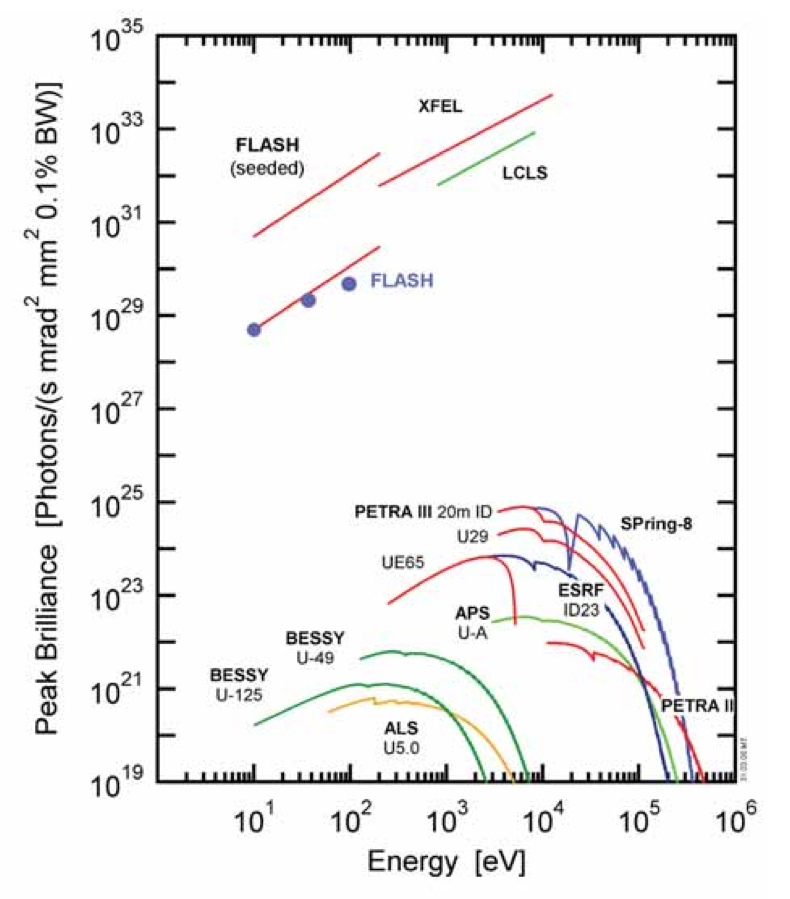
\includegraphics[width=.9\textwidth]{images/Other/XFEL-comparitive_energy-brightness.png}
  \caption{Plot of peak X-ray brilliance against energy for a range of current sources as well as the predicted values for EuXFEL (here labelled `XFEL'). The blue dots show measured peak brilliance for several energies at the existing FLASH facility, `FLASH (seeded)' is a proposed extension using a micro-bunch `seeded' electron beam.}
  \label{fig:xfel-brightness}
\end{figure}

% subsection x_ray_production_at_euxfel (end)
%%%%%%%%%%%%%%%%%%%%%%%%%%%%%%%%%%%%%%%%%%%%%%%%%%%
\subsection{Scientific Motivation} % (fold)
\label{sub:scientific_motivation}
There are two primary problems with more traditional synchrotrons: incoherent light and pulse length. As the light is produced in a long bunch of electrons it has no overall phase. This means that only samples that are crystalline (or can be crystallised, i.e.\ grown into a repeating pattern) can be imaged. Many structures form only poor crystals or can't form them at all. The X-ray pulse length that synchrotrons produce, whilst under normal operating conditions, are generally of order 10--100~ps~\cite{xfel_detector_requirements}. Obviously this places a lower limit on the speed of things that you can `film', again limiting the range of experiments that can be carried out. FELs solve both of these problems by producing coherent light that can have a very short pulse length, additionally because of the SASE process the peak brilliance of a FEL is vastly increased (see figure~\ref{fig:xfel-brightness}).

The primary aim of EuXFEL is to study conditions previously unseen in a laboratory setting. This aim is achieved through three core properties of EuXFEL: `coherence, ultra-high brilliance and time structure'~\cite{xfel_tdr} the combination of these gives access to three broad areas of study: the tiny, the fast and the extreme. Because of the limitations of incoherent light, pulse length and brilliance none of these regimes are easily studied at synchrotrons.

The imaging of the tiny relies on the wavelength of the light used being comparable to the scale of the structure to be imaged. At EuXFEL as well as having X-ray wavelengths sufficient to image molecules, due to the coherent nature of the light non-repeating structures can also be imaged unlike at traditional synchrotrons. Whilst the brilliance of the beam will destroy most samples very quickly, tests at FLASH show that enough time remains to produce a detailed image of the sample, even if it has not been crystallised. This means that larger structures can be imaged at an atomic scale (e.g.\ entire viruses) or structures that won't crystallise or only form very small, low quality crystals (e.g.\ protein membranes).

EuXFEL's time-structure, provides the potential of the second regime, speed. As each individual flash lasts less than \( \sim \)100~fs and each train comprising of 2,700 flashes it's possible to `film' processes as they occur. This will make it possible for researchers to understand what happens during a phase transition or when a material reverses its magnetisation by watching it happen in high detail and without suffering the motion-blur of slower systems.

The final regime, the extreme, is driven by EuXFEL's brilliance. Able to recreate intense temperatures and pressures EuXFEL can ue this to create environments not normally seen on Earth. For example: the propagation of shockwaves through a plasma or to image the stresses on a component under extreme magnetic fields.
% subsection scientific_motivation (end)
% section xfel_an_overview (end)
%%%%%%%%%%%%%%%%%%%%%%%%%%%%%%%%%%%%%%%%%%%%%%%  
\section{Detectors at EuXFEL} % (fold)
\label{sub:detectors_at_euxfel}
In order to achieve EuXFEL's scientific program a broad range of detectors are required. For almost all planned experiments there is a need to image the beam's interaction with the target, the standard solution to this is a 2D pixel detector. This type of detector consists of an array of light sensitive pixels that give both position and intensity information about the incident light, with minor reconstruction an image of the target can then be formed. The basic requirements for the 2D pixel detectors at EuXFEL are~\cite{xfel_tdr}:
\begin{description}
    \item[Swiftness] EuXFEL produces 27,000 X-ray pulses per second, the detector needs to be able to record a large number of these.
    \item[Dynamic range] In any one flash the number of photons received by any portion of the detector can vary massively (between 1 and \(10^5\) photons~\cite{lpd_manual}) this information needs to be preserved with a good signal to noise ratio by the detector.
    \item[Radiation resistance] When fully operational EuXFEL is intended to be used nearly continuously, so obviously any detector used has to be able to survive the harsh environment at the end of the beam-line.
\end{description}

There are currently three 2D pixel detectors being built for use at XFEL: Adaptive Gain Integrating Pixel Detector (AGIPD)~\cite{agipd_spec}, DEPFET Sensor with Signal Compression (DSSC)~\cite{dssc_spec} and Large Pixel Detector (LPD)~\cite{lpd_spec}. All three satisfy the above requirements through a variety of technologies.

The main differences between the three detectors are in their approach to the dynamic range: LPD and AGIPD both have three separate gain levels giving them the required range, whilst DSSC uses the non-linearity of its DEPFET to achieve a similar outcome. There are a few other significant differences: DSSC has hexagonal pixels (AGIPD and LPD have square); AGIPD uses dynamic switching to select the appropriate gain for each pixel before storing it in a single pipeline and LPD has an entire pipeline for each gain level (this means that when a narrower gain is required it can be set and all three pipelines used for storage). 

\subsection{The Large Pixel Detector (LPD)} % (fold)
\label{sub:the_large_pixel_detector_lpd}
LPD is a 2D, 1~Mega-pixel detector designed and build by a collaboration of the Rutherford Appleton Laboratory and Glasgow University in the UK. The detector is designed to be modular with a full 1~Megapixel being made up of 16 `supermodules', each supermodule contains a single Front End Module (FEM) that controls and reads out the 128 Application Specific Integrated Circuits (ASICs) each of which has 512 individual pixels i.e.\ each supermodule is 65,536 pixels divided between 128 ASICs and 1 FEM. It is the FEM that then communicates with the rest of EuXFEL via the Clock and Control Card (CCC) and the Train Builder (TB).
    
There are two lines specified for controlling the ASIC during operation: the system clock (\texttt{clk}) and the control (\texttt{cmd}). The FEM's CCC-interface is responsible for receiving the generic signals from the CCC and converting them to those expected by the ASIC. There are a large number of commands that the ASIC expects in order to function (a full list is given in appendix~\ref{app:asic_command_words}). These commands fall into a few general groups: starts, (no-)vetos\footnote{The ASIC actually uses a `trigger' rather than a `veto', but for consistency with the EuXFEL documentation we will use `no-veto' and `veto' to refer to \texttt{TRIGGER\_FLAG\_SET} and \texttt{NOP} respectively}, stops, resets, and testing. In each of these sets of commands there are generally two or tree individual command words that affect a specific component of the ASIC (e.g.\ reset the write pointer, start the trigger pointer). 
    
Each FEM uses a Xilinx~Virtex-5 Field Programmable Gate Array (FPGA) and two Xilinx~Spartan-3's for control and fan-out, the Virtex-5 has two softcore PowerPC440 processors that manage the resources on the FEM (e.g.\ configuring control registers). As well as the CCC-interface, firmware manages read-out of the ASIC; the ASICs' configuration and communication with the TB. The two Spartan-3 FPGAs are used primarily to co-ordinate fan-out of the signals to the ASICs.
% subsection the_large_pixel_detector_lpd (end)
% section detectors_at_euxfel (end)
\section{DAQ and control systems} % (fold)
\label{sec:daq_and_control_systems}
In a project the scale of EuXFEL there are a large number of different subsystems that need to communicate flawlessly in order to operate. Not only does a single common clock need to be distributed between all systems but it needs to compensate for the time to transmit a signal between the different components and how this latency may change depending on local conditions (e.g.\ the temperature). To maintain synchronicity there are several layers of timing and control system used at EuXFEL. The top-most layer is the master clock from which all other timing signals are derived. The master clock signal is distributed,  along with global information about the machine's status (e.g.\ the next bunch-train's ID), to the Timing Receiver (TR) cards. The 2D detectors use an additional layer (the CCC) to simplify their interface to the TR cards. The CCC removes information that is not needed by the 2D detectors and provides additional information that is received directly from other sub-systems (e.g.\ vetos). In addition to the CCC the 2D detectors share a second common interface, the Train Builder (TB) that provides a common method of storing and ordering data from each train.

The CCC has four primary functions in EuXFEL: 
\begin{enumerate}
  \item Distribution of the clocks required to maintain synchronicity with the rest of the machine.
  \item Control of the attached FEMS.
  \item Providing of veto information for each bunch.
  \item Collection of status information from the FEMs.
\end{enumerate}
In addition to these requirements the CCC can also operate in standalone mode (detached from a TR board) in order to facilitate testing and for use at other locations (e.g.\ LCLS). 

The CCC communicates with FEMs via RJ45 (see figure~\ref{fig:CCC_RJ45_diagram}), the four paired wires carry signals: clock, fast-command, veto and status. The clock signal is a \(\sim\)99~MHz derived from the TR and synchronised to the, \(\sim\)4.5~MHz, bunch clock, the fast command line carries information about each train whilst the veto line carries information on whether a bunch should be kept, the status line returns the received clock to indicate good connections.
\subsection{Clock and Control Card (CCC)} % (fold)
\label{sub:clock_and_control_card}
\begin{figure}[htbp]
  \centering
    \includegraphics[width=.9\textwidth]{images/Other/CCC_RJ45_diagram.png}
    % \includegraphics[width=.9\textwidth]{4_appendix_XFEL/images/Other/CCC_RJ45_diagram.png}
  \caption{The CCC RJ45 wiring diagram. Arrows on the inputs/outputs to FEE indicate signal direction, apart from the status line all are input to the FEE, i.e.\ the status line is the only line expected to send signals from the FEE to the CCC.}
  \label{fig:CCC_RJ45_diagram}
\end{figure}

% subsection clock_and_control_card (end)
\subsubsection{Clock signal} % (fold)
\label{sub:clock_signal}
Rather than a simple monotonic time structure, EuXFEL has two super-imposed patterns: the bunch trains and the bunches. The trains arrive at a rate of 10~Hz with each lasting only 600~\(\mu\)s but containing up to 2,700\( \times\)100~fs bunches, each separated from the next by \(\sim\)220~ns (i.e.\ a rate of \(\sim\)4.5~MHz), figure~\ref{fig:XFEL-time_structure} shows this.
\begin{figure}[htbp]
  \centering
    \includegraphics[width=.9\textwidth]{images/Other/XFEL-time_structure.png}
    % \includegraphics[width=.9\textwidth]{4_appendix_XFEL/images/Other/XFEL-time_structure.png}
  \caption{The timing structure of electrons at EuXFEL and the resultant X-ray pulses. }
  \label{fig:XFEL-time_structure}
\end{figure}

This timing structure forces the detectors to use the time between bunches for data read-out while during the bunch train they are limited to just storing data. This means that each detector is limited by the length of its on-ASIC pipeline with regards to how much data it can store (for LPD this is either 512 frames if using all three gain levels or 1536 if only using one). This structure also means there are two cycles that the detectors need to be synchronised to: the bunch clock (\(\sim\)4.5~MHz) and secondly the bunch-train clock (\(\sim\)10~Hz). Finally, in addition to these two machine-wide clocks there is the common CCC `fast clock' that is used for transmitting commands from the CCC which has a frequency of \(\sim\)99~MHz and is the clock that the ASIC works to.

Note: there is some vagueness as to the exact clock speeds used as, at time of writing a definitive value has yet to be decided on, the bunch clock is expected to remain between 4 and 5~MHz with the fast clock expected to be a simple divisor of this that results in a rate of roughly 100~MHz. 
% subsection clock_signal (end)
\subsubsection{Fast control} % (fold)
\label{sub:control_signal}
The fast control is used to convey information about each train. This information comes in four parts: when the next train will start, when it will stop, what its ID is and what bunch pattern should be used (see section~\ref{sub:veto_signal}, below). There is also a reset command to indicate that the ASIC and FEM should be reset to a known state. 

The expected use of the control signal is shown in table~\ref{tab:fast_commands}, a \texttt{START} signal arrives with attached train ID and bunch pattern ID, after some number of vetos the \texttt{STOP} signal is received. Rarely, either when there is a fault or if, for example, the detector's been switched off, the \texttt{RESET} signal will restore the FEM and ASIC to a prepared state.
\begin{table}[htbp]
  \begin{center}
  \begin{tabular}{c | c | c | c}
    Command  & Bits   & Payload & Description \\
    \hline   
    \multirow{2}{*}{START}    
             & \multirow{2}{*}{0b1100}
                      & Train ID (32b), bunch pattern  & \multirow{2}{*}{Start of the train} \\
             &        & ID (8b), checksum (8b)         & \\
    STOP     & 0b1010 & none                           & End of the train \\
    RESET    & 0b1001 & none                           & Reset the FEM and ASIC \\
    reserved & 0b1111 & n/a                            & n/a\\
  \end{tabular}
  \end{center}
  \caption{Specification of the fast command signals and their payloads.}
  \label{tab:fast_commands}
\end{table}
% subsubsection control_signal (end)
\subsubsection{Veto signals} % (fold)
\label{sub:veto_signal}
Given the previous discussion of the 2D detectors at EuXFEL (section~\ref{sub:detectors_at_euxfel}) it is obvious that it is unfortunately impossible for them to record all 2,700 bunches of the data, equally with a single linac being divided between five, and later ten, experimental stations not every detector will be receiving all of the bunches for every train anyway. To account for this there are two veto systems that allow the detectors to select which bunches they should record for processing: the `bunch pattern' and the `online veto'. Either of these two sources may veto a bunch so it is only recorded if \emph{neither} vetos it. 

The bunch pattern veto is derived from the global configuration of the machine: if, for example, the first half of the electron beam is being sent to another experimental station the detector will receive a pattern that tells it to veto that portion of the train. The patterns act as masks: for each bunch in a train the pattern states whether it should be vetoed or not. The bunch patterns are decided ahead of time, and a selection of patterns\footnote{Predicted to be fewer than 10.} are loaded when the FEM is configured, the bunch pattern to be used for each train is included in that train's header information as part of the start signal sent via the command line.

The online vetos are mainly situational, if the beam doesn't produce any X-rays or there is a fault then there is rarely any point taking data, in which case those bunches should be vetoed. These online vetos can have any source and the signals are supplied to a dedicated veto unit that is external to the CCC. The CCC will in turn pass on the veto or no-veto signal to the FEM of the detector, either with an attached bunch ID or with a fixed latency from the bunch in question depending on the specifications of the detector. Online vetos are what is received via the veto line and they have a format given in table~\ref{tab:veto_spec}, currently LPD makes no use of the bunch ID. The CCC promises that for every bunch either a VETO or a NOVETO signal will be sent, if neither is received then the interface will assume a NOVETO.
\begin{table}[htbp]
  \begin{center}
  \begin{tabular}{c|c|c|c}
    Command & Bits   & Payload                        & Notes\\
    \hline
    VETO    & 0b110  & \multirow{2}{*}{Bunch ID (8b)} & Veto this bunch \\
    NOVETO  & 0b101  &                                & Record this bunch \\
    reserved& 0b111  & n/a                            & n/a \\
  \end{tabular}
  \end{center}
  \caption{Veto signal specification.}
  \label{tab:veto_spec}
\end{table}
% subsection the_clock_and_control_card_ccc (end)
%%%%%%%%%%%%%%%%%%%%%%%%%%%%%%%%%%%%%%%%%%%%%%%
% section daq_and_control_systems (end)
\section{Firmware} % (fold)
\label{sec:firmware}
Firmware describes a broad range of technologies that bridge the divide between hardware (the physical chip and wires) and software (a program intended to run on a processor). Whilst firmware can often be used to refer to quiet complex programs run on embedded systems in this document it is used to refer to the specific logic loaded onto a programmable chip to configure its operation.

As discussed, the LPD FEM uses Virtex-5 FPGAs to run its firmware, FPGAs are made up of `slices' of logic that can be configured in order to create powerful systems. The general layout of a slice is a block of configurable logic attached to a Look Up Table (LUT) this combination provides basic logical manipulations followed by a brute force `if A then B' method of implementing the design. It's important to note that most modern FPGAs have additional dedicated slices that allows them to implement more specialised functions, examples include: digital signal processing, the previously discussed softcore processors, dedicated `Block RAM' (BRAM) etc. The specialised slices mean that software can be used to control configuration settings for the firmware natively which then can run without support from an operating system or creating a custom chip whilst also making use of large optimised structures like BRAM for storage.

\subsection{VHDL} % (fold)
\label{sub:vhdl}
There are a variety of languages for writing firmware, the one used for LPD is VHSIC\footnote{Very High Speed Integrated Circuit} Hardware Description Language (VHDL). VHDL works by describing the expected operation of various discrete blocks within the firmware, these descriptions are then translated (synthesised) into bit-code that, in the case of FPGAs will tell the chip how to configure itself.

Whilst a detailed description of the language are beyond the scope of this document there are several attributes of it that are required to understand the following discussions. The key difference is that VHDL is \emph{description} language. This means that the code exists to describe the mapping from inputs to outputs, how this is actually implemented is left to the compiler. The upshot of this system is that depending on the target being compiled for (e.g.\ FPGA, ASIC, etc.) you can get very different implementations of the same code.

% Whilst a detailed description of the language are beyond the scope of this document there are several attributes of it that are required to understand the following discussions. The first major feature of VHDL to be understood is that it is a \emph{description} language as such the specification makes few guarantees about how any particular block of logic will be implemented as the it ultimately only defines what the inputs and the outputs of a block are, consequentially the same code may produce very different results depending on the synthesiser used and the intended target (e.g.\ FPGA, ASIC, etc.).

The slice-based architecture of FPGAs means that many designs are synthesised as `apply logic to signals' then `look up value of signals in table' and finally `output value stored in table'. The result of this system is that most designs are split into two groups of components the `state-machine' and the `memory'. A state-machine is a set of states with attached conditions, the inputs to the state-machine determine which state should be selected and then that state determines what the output should be, the memory stores any persistent information needed by the state-machine either as input, or output. Throughout CCC-interface firmware there are examples of this where a state-machine implements the logic and a BRAM provides large scale storage.

In VHDL, blocks of code (called `entities') are defined by their name, ports and generics; entities represent a cohesive unit of logic, for example a state-machine. Ports represent in or out-bound signals\footnote{VHDL also specifies `inout' as a bi-directional port but they are not used here.} to that entity, these can either be single or grouped into vectors. The generics of an entity describe constant values associated with it; they can be changed on a per-synthesis scale but not by the firmware itself. Generics are mainly used in the design to specify reset values for registers and values that shouldn't be changeable at run time, but may need to change between systems (e.g.\ delays). 

VHDL specifies two broad classes of value that can be used for ports: signals and vectors, a signal is a single bit of information whilst a vector is a collection of bits in some order. VHDL's basic signal type is called `std\_logic' (sl). std\_logic is generally used for transfer of the boolean values (`1' or `0') but it can also take several other values\footnote{`L', `H', `U', `W', `X', `Z' and `-'.} that better describe the ultimately analogue reality of hardware signals e.g.\ the value `L' specifies a weak signal that should probably be low. The vector form of std\_logic is a `std\_logic\_vector' (slv) that is ordered `X (up)to Y' or `Y downto X', if the slv is converted to a numeric type (e.g.\ an integer) then this ordering determines the `endedness'. E.g.\ if an slv (3 downto 0) is 0b1000 then it has an integer value of 8, the same value but with ordered reversed (i.e.\ 3 to 0) has an integer of 1. Throughout this document order is denoted using parenthesis e.g.\ slv~(3:0) is a std\_logic\_vector~(3~downto~0) while slv~(0:3) is (3~to~0).
% subsection vhdl (end)
%%%%%%%%%%%%%%%%%%%%%%%%%%%%%%%%%%%%%%%%%%%%%%%%%%%
% section firmware (end)
%%%%%%%%%%%%%%%%%%%%%%%%%%%%%%%%%%%%%%%%%%%%%%%
